% To convert to svg
% lualatex --output-format=dvi mother.tex
% dvisvgm mother.dvi
% \documentclass[dvisvgm]{minimal}		%uncomment to convert to svg

\documentclass[border=0]{standalone}
\usepackage{tikz}
\usetikzlibrary{calc,shapes.geometric,through,intersections}
\usepackage{xcolor}
\definecolor{highlight2}{HTML}{99cc99}
\usepackage{xkcdcolors}
\begin{document}
    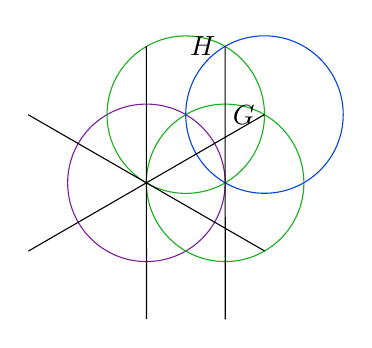
\begin{tikzpicture}
        \coordinate (O) at (0,0);
        \draw[xkcdPurple] (O) circle (1);
        \draw[name path=P,xkcdGreen] (0:1) circle (1);
        \draw[name path=Q,xkcdGreen] (60:1) circle (1);
        \path [name intersections={of=P and Q,by={[label=left:$G$]G}}];
        \draw[name path=R,xkcdBlue] (G) circle (1);
        \draw ($(O)!-1!(G)$) -- (G);
        \draw ($(O)!-1!($(O)!1!60:(G)$)$) -- ($(O)!1!60:(G)$);
        \draw ($(O)!-1!($(O)!1!120:(G)$)$) -- ($(O)!1!120:(G)$);
        \path [name intersections={of=R and Q,by={[label=left:$H$]H}}];
        \draw (H) -- ($(O)!1!-120:(H)$);
    \end{tikzpicture}
\end{document}
